\chapter{WATER QUALITY}
\label{ch:wat:qual}

\section{  Introduction}

 Since release 7.0, \telemac{2d} offers the possibility to simulate simple water quality processes. We give here some preliminary elements about theory, implementation and use of the water quality software \waqtel. This code was originally extracted from TRACER the water quality module of the 1D Mascaret system.

\section{ Theoretical aspects}

 \waqtel offers the use of 6 water quality (WAQ) processes. These processes generate source terms that are added to the advection-diffusion equation resolved in Telemac-2d. These processes are the following:

\begin{itemize}
\item  O2 module:  which gives the evolution of oxygen O2 in the flow and accounts for the interaction with the organic load and ammoniacal load. This module is simple since it does not take into consideration all the complexity of biological phenomena linked to the production, the elimination and the transport of oxygen. For more details about this process, reader is invited to the following manual and references therein (\cite{El-Kadi2012}).

\item  Biomass module:  it allows the computation of the algal biomass. It estimates the vegetal colonization as a function of several parameters such as sunshine, water temperature, ratio of renewing of water etc. This module introduces and uses 5 tracers:

\begin{enumerate}
\item  phytoplanktonic biomass (PHY)

\item  dissolved mineral phosphorus PO${}_{4}$

\item  degradable phosphorus assimilated by phytoplankton (POR)

\item  dissolved mineral nitrogen assimilated by phytoplankton (NO${}_{3}$ )

\item  degradable nitrogen assimilated by phytoplankton (NOR)
\end{enumerate}

\item  Eutro module:  this module describes the oxygenation of a river. It is much more complex than the O${}_{2}$ module since it takes into account vegetal photosynthesis and nutrients and their interactions with phytoplankton. This module introduces 8 tracers:
\begin{enumerate}
\item  phosphorus assimilated by phytoplankton (POR)

\item  dissolved oxygen O${}_{2}$

\item  phytoplanktonic biomass (PHY)

\item  dissolved mineral phosphorus (PO${}_{4}$)

\item  degradable dissolved mineral nitrogen assimilated by phytoplankton (NO${}_{3}$)

\item  degradable nitrogen assimilated by phytoplankton (NOR)

\item  ammoniacal load (NH${}_{4}$)

\item  organic load (L)
\end{enumerate}

     These tracers are in mg/l, except biomass which is given in $\mu$g.

\item  Micropol module:  this module gives the evolution of micro-pollutants (radio-elements or heavy metals) in the main locations in river flows i.e. water, suspended load and bed sediments. This module introduces 5 tracers:
\begin{enumerate}
\item  suspended sediments (SS)

\item  bed sediments (BS), which are considered fix (not advected neither dispersed)

\item  micro-pollutant species in dissolved form

\item  part absorbed by suspended sediments

\item  part absorbed by bed sediments
\end{enumerate}

\item  Thermic module: this module computes the evolution of water temperature as a function of heat exchange balance with atmosphere. Only the exchanges with atmosphere are considered, those with lateral boundaries and with the bed are neglected or have to be given in the boundary conditions file.
\item The Aquatic Ecodynamics library (AED2): this library is fully developed by an australian consortium (see website for more information http://aed.see.uwa.edu.au/research/models/AED/ ).
\end{itemize}


\section{ Practical aspects}



 To activate the water quality module, the logical key-word \textit{WATER QUALITY} must be set to TRUE (default= FALSE).  In telemac2D, a new dictionary is created and fully dedicated to water quality applications. The description of this new dictionary will be the subject of a separate manual. \telemac{2d} will not read automatically this dictionary, unless the key-word \textit{WAQ DICTIONARY} is used. This key-word is the path to dictionary. To introduce WAQ parameters, a separate steering file is necessary. It is read with the use of key-word \textit{WAQ STEERING FILE}. In the next section which is dedicated to water quality, all the key-words to be introduced to the water quality steering file will be written in \textbf{\textit{BOLD AND ITALIC UPPER CASE.}}

 Depending on the WAQ module, \telemac{2d} increases automatically the number of tracers of the model. In fact, the total number of tracers (variable ntrac) is increased by 3 (for O2 process), by 5 (for Biomass and Micropol processes) or by 8 (for Eutro process). For the Thermic module, the number of tracers is increased only if no temperature is present in the set of tracers already existing in the model.

 Some general parameters can also be chosen for any water quality process. For instance, user can give a title for the study by using \textbf{\textit{WAQ CASE TITLE}}. He can introduce water density \textbf{(\textit{WATER DENSITY}}), viscosity of water \textbf{\textit{(KINEMATIC WATER VISCOSITY}}).


\subsection{  The meteo file}
\label{subs:meteo:file}
 Most of the water quality processes are tightly linked to meteorological data on the domain. Besides the specific treatment for wind, atmospheric pressure and rain described in section \ref{sec:param:met:phen}, water quality needs different meteorological data such as nebulosity, air temperature, evaporation pressure etc. Hereafter we give an example of meteo file (see Table \ref{tab:meteo}). User can edit this file and add new parameters, however, in this case, he must edit subroutine meteo.f consequently.

\begin{table}
    \centering
  \begin{tabular}{|l|c|c|c|c|c|c|c|c|}
     \hline \hline
     % after \\: \hline or \cline{col1-col2} \cline{col3-col4} ...
     Time & $T_{air}$ & $P_{vap}$ & $Wind speed$ & Wind Dir. & Nebulo. & Ray. & $P_{atm}$ & Rain \\
     \hline \hline
     sec & $deg C $ & hPa & m/s & deg & Octa & $W/m^2$ & mbar & mm \\
     \hline \hline
     0 & 20 & 10 & 0 & 0.70 & 5 & 160 & 1012.7 & 0 \\
     3600 & 20 & 10 & 0 & 0.70 & 5 & 160 & 1012.7 & 0 \\
     7200 & 20 & 10 & 0 & 0.70 & 5 & 160 & 1012.7 & 0 \\
     \hline
   \end{tabular}
  \caption{Example of meteo data file }\label{tab:meteo}
\end{table}


\subsection{ O2 module}
\label{subs:O2:mod}


 The O2 module is a simple model that describes the evolution of the oxygen density in the water. It is activated by setting \textbf{\textit{WATER QUALITY PROCESS}}\textit{ = 1}. It offers the advantage of being simple and then easy to calibrate. Indeed, since some important parameters are kept constant (such as vegetal respiration \textbf{\textit{VEGETAL RESPIRATION R}}, benthic demand \textbf{\textit{BENTHIC DEMAND}}), only 8 parameters have to be introduced (and, if necessary calibrated). The use of this module is, consequently, recommended for short time periods (several days)

 O2 module uses 3 tracers:

\begin{enumerate}
\item  Dissolved oxygen O2 (mgO2/l)

\item  Organic load L (mgO2/l)

\item  Ammoniacal load NH4 (mgO2/l)
\end{enumerate}

 These tracers are hence, advected and dispersed in the whole water mass and their evolution obeys the advection-diffusion equation linked to external and internal source terms.


\paragraph{ The dissolved oxygen}

 The dissolved oxygen density is influenced by the following factors:

\begin{itemize}
\item  4 factors consuming oxygen:

\begin{enumerate}
\item  Organic load L
\item  Ammoniacal load
\item  Benthic demand
\item  Vegetal respiration
\end{enumerate}

\item  2 factors producing oxygen
\begin{enumerate}
\item  Photosynthesis

\item  Reaeration
\end{enumerate}
\end{itemize}
 We will introduce briefly how are estimated the source terms linked to these six factors.




{\bf  The benthic demand}

 The benthic demand is provided by the user in gO2/m2/day using the key-word \textbf{\textit{BENTHIC DEMAND}} (default 0.1). It is then corrected with water temperature T like:
\[{BEN}_T={BEN}_{T20{}^\circ C}{\left(1.065\right)}^{T-20}\]
Where T is given in Celsius degree using the key-word \textbf{WATER TEMPERATURE} (default 7${}^\circ$C). This value of temperature is useful when the temperature is not considered as a tracer in the model; otherwise, the real temperature is taken into account.




{\bf  Vegetal respiration}

 It is given directly by the user with key-word \textbf{\textit{VEGETAL RESPIRATION R}} (default 0.06 mgO${}_{2}$/d/l).


{\bf  Photosynthesis P}

 Photosynthesis P (in mgO${}_{2}$/d/l) depends on algae density, water depth and sunlight. It is very often between 0.3 and 9 mgO${}_{2}$/d/l. for O${}_{2}$ module, it is given by the user with the key-word \textbf{PHOTOSYNTHESIS P} (default 1. mgO${}_{2}$/d/l).


{\bf  Reaeration}

 It is the gain oxygen through the free surface of water. It is due to 2 main raisons:  the natural reaeration and the weir reaeration.

\begin{itemize}
\item  Natural reaeration: it can be seen at a macroscopic level as a term which is linearly dependent on (Cs-[O2]), where Cs is O2 saturation density of water (given through key-word \textbf{\textit{O2 SATURATION DENSITY OF WATER (CS)},} default 11. mg/l) and [O2] is the O2 density. For instance Cs = 9mg/l at 20${}^\circ$C.  We get finally:

 Natural reaeration = K2(Cs-[O2]),

 Where K2 (given in 1/d) is an empirical parameter which can be computed using 4 empirical laws. The choice of the law is given by the keyword \textbf{\textit{FORMULA FOR COMPUTING K2}} which can have the following values:

\begin{itemize}
\item  0~: K2 constant, its value is given by keyword\textbf{ \textit{K2 REAERATION COEFFICIENT}} (default 0.9)

\item  1: formula of the Tenessee Valley Authority: $K_2=5.23\ Uh^{-1.67}$, with U is the velocity and h is the water depth at each point of the mesh.

\item  2: formula of Owens et al.  $K_2=5.33\ U^{0.67}h^{-1.85}$.

\item  3: formula of Churchill et al. $K_2=0.746\ U^{2.695}h^{-3.085}J^{-0.823}$, where J is the head loss .

\item  4: formula of O'Connor \& Dobbins~: $K_2=3.9U^{0.5}h^{-1.5}$

\item  5: formula mixing the last 3 formulae $K_2=5.33\ U^{0.67}h^{-1.85}$ if h$<$0.6; $K_2=0.746\ U^{2.695}h^{-3.085}J^{-0.823}$ if h$<$12U-6.6; $K_2=0.746\ U^{2.695}h^{-3.085}J^{-0.823}\ elswhere$
\end{itemize}

\begin{figure}
  \centering
  % Requires \usepackage{graphicx}
  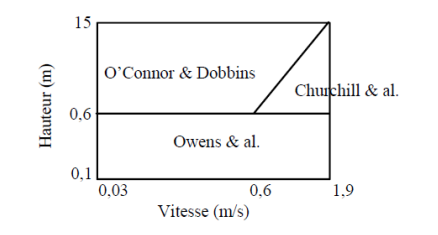
\includegraphics[width=8cm]{./graphics/k2diagram.png}\\
  \caption{choice of the K2 formula depending on hydrodynamics of the flow}\label{k2choice}
\end{figure}


 Since these formulae are valid for a temperature of 20${}^\circ$C, the value of K2 is corrected like:
\[K_2={\left(K_2\right)}_{20{}^\circ C}\ {\left(1.024\right)}^{T-20}\]


 The oxygen density at saturation Cs can be estimated using the temperature of water (at 20${}^\circ$C, Cs=9 mg/l). Hence if the temperature in the model is varying with time (for example when Thermic Module is activated), Cs can be estimated with different ways using the key-word \textbf{\textit{FORMULA FOR COMPUTING CS}} (default 0) which can have the following values:

\begin{itemize}
\item  0: constant value given by \textbf{\textit{O2 SATURATION DENSITY OF WATER (CS)}} (default = 11mg/l)

\item  1: Formula of Elmore \& Hayes:
\[C_s=14.652-0.41022T+0.00799T^2-7.7774.{10}^{-5}T^3\]

\item  2: Formula of Montgomery:
\[C_s=468/(31.6+T)\]
\end{itemize}

\item  Reaeration at weirs: for the O2 process, a reaeration of the water due to the existence of weirs is implemented. The water oxygen concentration is increased when crossing from one side of a weir to the other side. The raise of the concentration is managed through the key-words \textbf{\textit{WEIR REAERATION COEFFICIENT RS}} and \textbf{\textit{FORMULA FOR COMPUTING RS}} which can have 5 options (see \cite{El-Kadi2012} for theoretical details):
\begin{itemize}
\item  0: RS is constant, in this case RS is given by \textbf{\textit{WEIR REAERATION COEFFICIENT RS }}(default 1.)

\item  1: formula of Gameson 1

\item  2: formula of Gameson 2

\item  3: formula of WRL1

\item  4: formula of WRL2
\end{itemize}
\end{itemize}




\paragraph{  Organic load L}

 The evolution of the organic load density [L] in time is assumed to be with a first order law:
\begin{equation*}
 F([L]) = K_1 [L]
\end{equation*}
 Where $K_1$ is a constant that describes the kinetic of degradation of the organic load. It is given using the key-word \textbf{\textit{CONSTANT OF DEGRADATION OF ORGANIC LOAD K1}} (default 0.25 per day).  The organic load is in mgO$_2$/l.


\paragraph{ Ammoniacal load}

 The ammoniacal load $NH_4$, which is also consuming oxygen, has a density varying in time with a first order law given by:
\begin{equation*}
 F([NH{}_{4}]) = K_4 [NH{}_{4}]
\end{equation*}
 Where $K_4$ is a constant of nitrification kinetic. It is given by \textbf{\textit{CONSTANT OF NITRIFICATION KINETIC K4}}\textit{ }(default 0.35). In this module, $K_4$ is assumed to be constant and independent of remaining variables.


\paragraph{ Final source terms}

 The oxygen density is varying under the influence of sources with respect to the following law:
\begin{equation*}
F\left([O_2]\right)= K_2\left(C_s-[O_2]\right)-K_1\left[L\right]-K_4\left[NH_4\right]+P-R-\frac{BEN}{h}
\end{equation*}

\paragraph{ Example of steering file}

 To activate the water quality module we give here the set of key-words to include in the steering file of \telemac{2d}:
\begin{lstlisting}[language=bash]
/------------------------------------------------------
  WATER QUALITY
/------------------------------------------------------
WATER QUALITY           = YES
WAQ STEERING FILE    = 'waq\_steer.cas'
WAQ DICTIONARY         = 'waqtel.dico'
\end{lstlisting}
We give hereafter an example of WAQ steering file with the use of O${}_{2}$ process:
\begin{lstlisting}[language=bash]
/WAQ STEERING FILE
/---------------------------------------------------------
/GENERAL PARAMETERS:
/---------------------------------------------------------
WAQ CASE TITLE                = 'WAQ O2: VALIDATION CASE'
WATER DENSITY                 = 1000.
KINEMATIC WATER VISCOSITY     = 1.E-6
WATER QUALITY PROCESS         = 1
/   OPTIONS ARE :
/       1- O2 PROCESS
/       2- BIOMASS PROCESS
/       3- EUTRO PROCESS
/       4- MICROPOL PROCESS
/       5- THERMIC PROCESS
/-----------------------
//
// O2 PROCESS
//
/-----------------------
CONSTANT OF DEGRADATION OF ORGANIC LOAD K1 = 0.25
CONSTANT OF NITRIFICATION KINETIC K4       = 0.35
PHOTOSYNTHESIS P                           = 1.
VEGERAL RESPIRATION R                      = 0.06
WATER TEMPERATURE                          = 20.
/ In case of existence of weirs uncomment the following lines:
/WEIR REAERATION COEFFICIENT RS'
/FORMULA FOR COMPUTING RS'
//GIVES HOW TO CUMPUTE THE WEIR REAERATION COEFFICIENT RS
//OPTIONS ARE:
//  0- RS CONSTANT, IN THIS CASE RS=1.0
//  1- FORMULA OF GAMESON 1
//  2- FORMULA OF GAMESON 2
//  3- FORMULA OF WRL 1
//  4- FORMULA OF WRL2
/COEFFICIENTS A AND B FOR RS FORMULA'
\end{lstlisting}

\subsection{ The thermic module}
\label{subs:therm:mod}
 For a majority of water quality processes, the interaction with atmosphere is a key parameter. The neighboring conditions are taken into account through a meteorological file like the one described in section \ref{subs:meteo:file}. It is important to underline that the data contained in this file can vary depending on the considered case. The subroutine meteo can be edited by user to customize it to his specific model.

 The evolution of temperature of water is tightly linked to heat fluxes through the free surface. These fluxes (in W/m2) are of 5 natures:

\begin{itemize}
\item  Sun ray flux RS

\item  Atmospheric radiation flux RA

\item  Free surface radiation flux RE

\item  Advection heat flux CV

\item  Heat flux due to evaporation CE
\end{itemize}

 The final balance of (surface) source terms is given by
\[s_{surf}=RS+RA-RE-CV-CE\]
We will give a brief description for each of these terms, for more details see \cite{El-Kadi2012}. This surface source term is treated explicitly in \telemac{2d}, the following term is added in the explicit source term of advection-diffusion equation of tracer$\frac{S_{surf}}{\rho C_pH}$.


\paragraph{ Sun ray flux RS}

 Sun ray flux is simply provided in the meteo file. In a majority of cases, when no measurements are not available, this flux is estimated using the method of Perrin \& Brichambaut (\cite{El-Kadi2012}), which uses the cloud cover of the sky that varies during the day (function of time). So far, this flux is considered constant in space.  For more real cases, user is invited to use the ``heat exchange'' module (in folder sources/telemac3d). A sun ray flux varying in space, common between \telemac{2d} and \telemac{3d} will be implemented in next releases.


\paragraph{ Atmospheric radiation RA}

 The atmospheric radiation RA is estimated with meteorological data collected at the ground level. It takes into account energy exchanges with the ground, water (and energy) exchanges with the underground, etc. In this module, RA is estimated mainly by the air temperature, like:
\begin{equation*}
RA=e_{air}\sigma\left(T_{air}+273.15 \right)^4\left(1+k\left(\frac{c}{8}\right)^2 \right)
\end{equation*}
 Where $e_{air}$ is a calibrating coefficient given the key-word \textbf{\textit{COEFFICIENTS FOR CALIBRATING ATMOSPHERIC RADIATION} }(default 0.75). $\sigma$ is the constant of Stefan-Boltzmann (5.67.10${}^{-8}$ Wm${}^{-2}$K${}^{-4}$). Tair is air temperature given in the meteo file. k is coefficient that represents the nature of clouds, it has a mean value of 0.2 (key-word \textbf{\textit{COEFFICIENT OF CLOUDING RATE}}). However, it varies like indicated in Table \ref{tab:kcloud}.
\begin{table}
  \centering
  \begin{tabular}{|l|c|}
     \hline
     Type of cloud & k \\
     \hline \hline
     Cirrus & 0.04 \\
     Cirro-stratus & 0.08 \\
     Altocumulus & 0.17 \\
     Altostratus & 0.2 \\
     Cumulus & 0.2 \\
     Stratus & 0.24\\
     \hline
   \end{tabular}
  \caption{Values of k depending on cloud type}\label{tab:kcloud}
\end{table}



\paragraph{  Free surface radiation RE}

 The available water is assumed to be a grey body. Radiation generated by this grey body through the free surface is given by:
\begin{equation*}
RE=e_{eau}\sigma\left(T_{eau}+273.15 \right)^4
\end{equation*}
where T${}_{eau}$ is the mean water temperature in ${}^\circ$C. T${}_{eau}$ is given by the key-word \textbf{\textit{WATER TEMPERATURE}} (default 7${}^\circ$C). e${}_{eau}$ is a calibration coefficient which depends on the nature of the site and obstacles around it. This coefficient is given with \textbf{\textit{COEFFICIENTS FOR CALIBRATING SURFACE WATER RADIATION}} (default 0.97). For instance, for a narrow river with lots of trees on its banks, e${}_{eau}$ is around 0.97, for large rivers or lakes it is about 0.92.


\paragraph{ Advection heat flux CV}

 This flux is estimated empirically:
\begin{equation*}
CV=\rho_{air}Cp_{air}\left(a+bV \right)\left(T_{eau}-T_{air} \right)
\end{equation*}
 where $\rho_{air}$ is the air density obtained by ${\rho }_{air}=\ \frac{100\ P_{atm}}{\left(T_{air}+273.15\right)287}$ where P${}_{atm}$ is the atmospheric pressure, introduced in the meteo file or using the key-word \textit{VALUE OF ATMOSPHERIC PRESSURE} (default 100~000 Pa) (this is a key-word of \telemac{2d}). Cp${}_{air}$ is the air specific heat (J/kg${}^\circ$C) given by \textbf{\textit{AIR SPECIFIC HEAT}} (default 1002), V is the wind velocity (m/s) and a, b are empirical coefficients to be calibrated. Theirs values are very close to 0.0025, but they can be changed using \textbf{\textit{COEFFICIENTS OF AERATION FORMULA}} (default (0.002, 0.0012)).


\paragraph{ Evaporation heat flux CE}

 It is given by the following empirical formula:
\begin{equation*}
CE=L\rho_{air}\left(a+bV \right) \left(H^{sat}-H \right)
\end{equation*}
 where L=2500900-2365T${}_{water}$ is the vaporization latent heat (J/Kg), $H^{sat}=\frac{0.622P^{sat}_{vap}}{P_{atm}-0.378P^{sat}_{vap}}$ is the air specific moisture (humidity) at saturation (kg/kg), $H=\frac{0.622P_{vap}}{P_{atm}-0.378P_{vap}}$ is the specific humidity of air (kg/kg), P${}_{vap}$ is the partial pressure of water vapour in the air (hPa=10${}^{5}$Pa) which is given in the meteo file. $P^{sat}_{vap}$ is the partial pressure of water vapour at saturation (hPa) which is estimated with :
\begin{equation*}
P^{sat}_{vap}=6.11exp\left(\frac{17.27T_{eau}}{T_{eau}+237.3} \right)
\end{equation*}
 when H${}^{sat}<$H, the atmospheric radiation RA is corrected by multiplying it with 1.8.


\paragraph{ Example of steering file}

 To activate the water quality module we give here the set of key-words to include in the steering file of \telemac{2d}:
\begin{lstlisting}[language=bash]
/------------------------------------------------------
  WATER QUALITY
/------------------------------------------------------
WATER QUALITY           = YES
WAQ STEERING FILE    = 'waq\_steer.cas'
WAQ DICTIONARY         = 'waqtel.dico'
\end{lstlisting}
 We give hereafter an example of WAQ steering file with the use of Thermic process:
\begin{lstlisting}[language=bash]
/WAQ STEERING FILE
/--------------------------------------------------------------
/GENERAL PARAMETERS:
/--------------------------------------------------------------
WAQ CASE TITLE                = 'WAQ THERMIC: VALIDATION CASE'
WATER DENSITY                 = 1000.
KINEMATIC WATER VISCOSITY     = 1.E-6
WATER QUALITY PROCESS         = 5
/   OPTIONS ARE:
/       1- O2 PROCESS
/       2- BIOMASS PROCESS
/       3- EUTRO PROCESS
/       4- MICROPOL PROCESS
/       5- THERMIC PROCESS
/--------------------------------------------------------------
//
//THERMIC PROCESS
//
WATER SPECIFIC HEAT                                  = 4180.
AIR SPECIFIC HEAT                                    = 1002.
COEFFICIENTS OF AERATION FORMULA                = 0.0025;0.0025
COEFFICIENT OF CLOUDING RATE                         = 0.2
COEFFICIENTS FOR CALIBRATING ATMOSPHERIC RADIATION   = 0.85
COEFFICIENTS FOR CALIBRATING SURFACE WATER RADIATION = 0.97
\end{lstlisting}
